% DAQCNN Pipeline Schematic
% Standalone TikZ figure. Compile with: pdflatex daqcnn_pipeline.tex
\documentclass[tikz,border=10pt]{standalone}

\usepackage{amsmath,amssymb,amsfonts}
\usepackage{xfrac}
\usepackage{xcolor}
\usepackage{mathptmx}        % Times Roman, matches IEEEtran body font
\usepackage{tikz}
\usetikzlibrary{positioning, shapes.geometric, shapes.misc, arrows.meta,
                calc, fit, backgrounds, decorations.pathreplacing,
                decorations.markings, patterns, shadows}

%====================  COLOUR PALETTE  ====================%
\definecolor{qblue}      {HTML}{2C5A9E}
\definecolor{qblueDeep}  {HTML}{1F3F70}
\definecolor{qblueMid}   {HTML}{6A8EC4}
\definecolor{qblueLight} {HTML}{D6E2F3}
\definecolor{qblueFade}  {HTML}{EEF3FB}
\definecolor{corange}    {HTML}{C66C2C}
\definecolor{corangeMid} {HTML}{E29762}
\definecolor{corangeLight}{HTML}{FBEDDD}
\definecolor{corangeFade}{HTML}{FDF7EF}
\definecolor{txt}        {HTML}{1E2330}
\definecolor{txtSoft}    {HTML}{555866}
\definecolor{accent}     {HTML}{B23064}
\definecolor{bondCol}    {HTML}{707481}
\definecolor{convA}      {HTML}{D58A52}
\definecolor{convB}      {HTML}{CC7434}
\definecolor{convC}      {HTML}{B05E22}
\definecolor{fcCol}      {HTML}{93501F}

\begin{document}
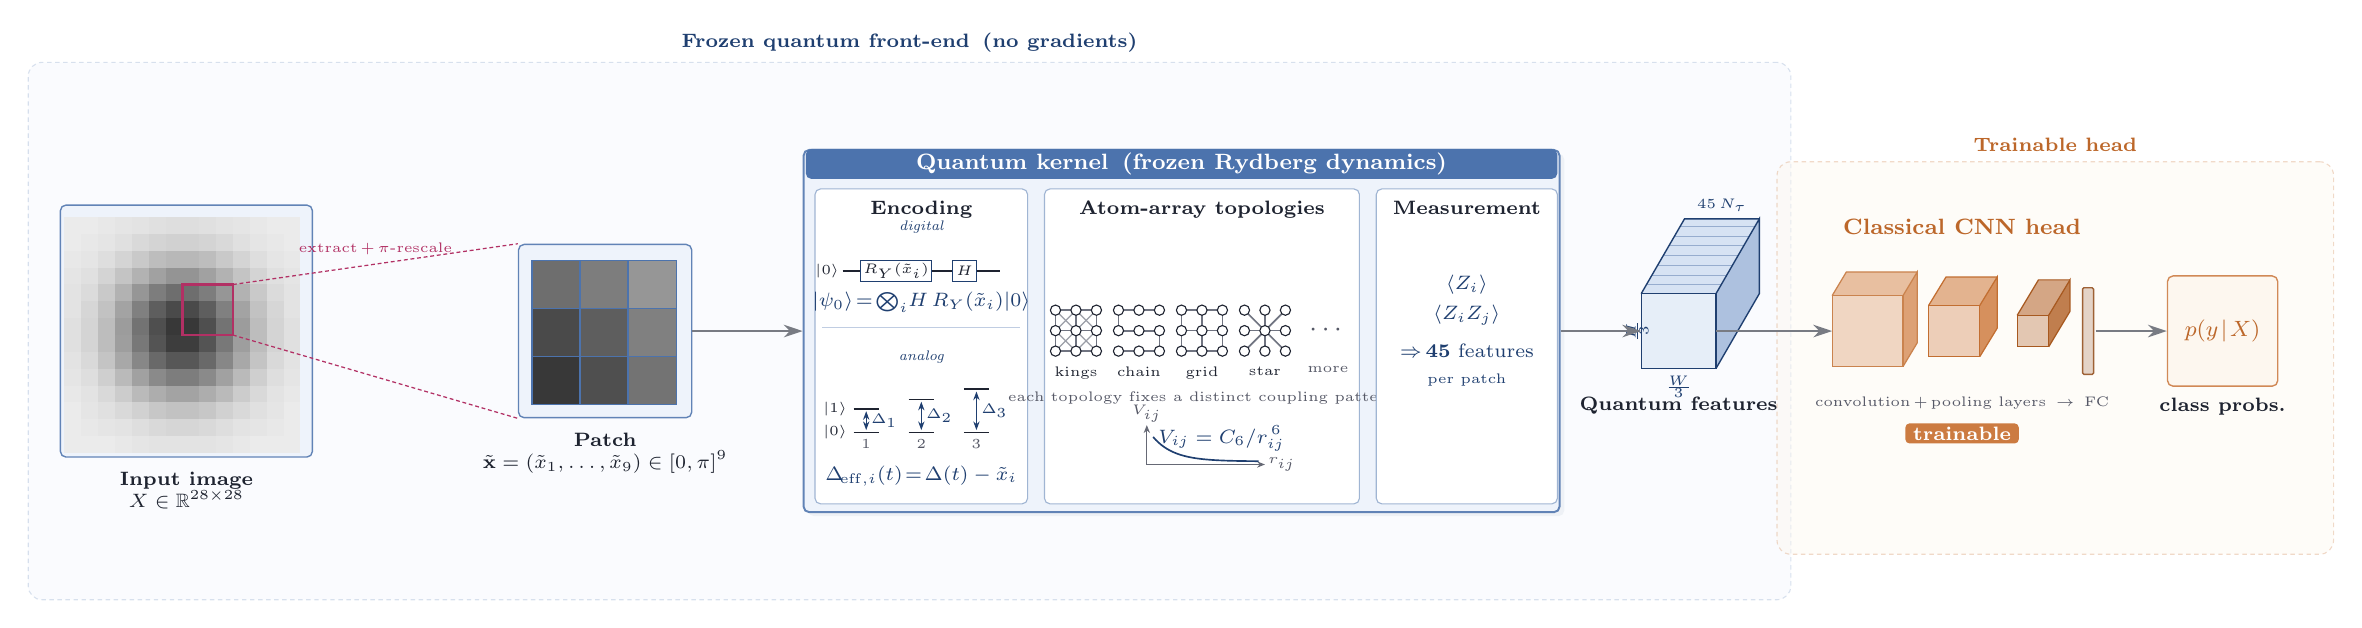
\begin{tikzpicture}[
    >={Stealth[length=2.4mm,width=1.6mm]},
    font=\small,
    every node/.style={text=txt, inner sep=2pt},
    arr/.style={->, draw=txt!60, line width=0.6pt},
    panel/.style={rectangle, rounded corners=2pt, align=center, line width=0.5pt},
    qpanel/.style={panel, draw=qblue!75, fill=qblueFade},
    cpanel/.style={panel, draw=corange!80, fill=corangeFade},
    innerq/.style={panel, draw=qblue!45, fill=white, line width=0.4pt},
    lab/.style={font=\scriptsize, text=txtSoft, align=center, inner sep=1pt},
    lab2/.style={font=\scriptsize, text=txt, align=center, inner sep=1pt},
    zone/.style={rounded corners=5pt, line width=0.4pt, dash pattern=on 1.6pt off 1.3pt},
    atomNode/.style={circle, draw=txt, fill=white, line width=0.35pt,
                     minimum size=1.4mm, inner sep=0pt},
    smallAtom/.style={circle, draw=txt, fill=white, line width=0.4pt,
                      minimum size=1.3mm, inner sep=0pt},
    gateBox/.style={draw=qblueDeep, fill=white, line width=0.35pt,
                    minimum height=2.6mm, font=\tiny, inner xsep=1pt, inner ysep=0pt},
]

%====================================================================
%  STAGE 1 — INPUT IMAGE (large, blob-like) WITH SELECTION + ZOOM
%====================================================================
\node[qpanel, minimum width=32mm, minimum height=32mm] (image) at (0,0) {};

% Procedural Gaussian-blob image (14x14 pixels) — clean blob, no noise so the
% patch view can exactly reproduce the selection region.
\foreach \i in {0,...,13}{
  \foreach \j in {0,...,13}{
    \pgfmathsetmacro{\dd}{((\i-6.5)*(\i-6.5)+(\j-6.7)*(\j-6.7))/15}
    \pgfmathsetmacro{\base}{8+72*exp(-\dd)}
    \pgfmathtruncatemacro{\valInt}{max(2,min(95,\base))}
    \fill[black!\valInt]
      ($(image.south west)+(0.06+0.214*\i, 0.06+0.214*\j)$) rectangle ++(0.214,0.214);
  }
}

\node[lab2, below=1.4mm of image, font=\scriptsize]
  {\textbf{Input image}\\$X\in\mathbb{R}^{28\times 28}$};

% --- 3x3 selection box on the image
\coordinate (selLL) at ($(image.south west)+(0.06+0.214*7.0, 0.06+0.214*7.0)$);
\coordinate (selUR) at ($(image.south west)+(0.06+0.214*10.0,0.06+0.214*10.0)$);
\coordinate (selLR) at ($(image.south west)+(0.06+0.214*10.0,0.06+0.214*7.0)$);
\coordinate (selUL) at ($(image.south west)+(0.06+0.214*7.0, 0.06+0.214*10.0)$);
\draw[accent, line width=0.85pt] (selLL) rectangle (selUR);

%====================================================================
%  STAGE 2 — ZOOMED PATCH (magnification cone from selection)
%====================================================================
\node[qpanel, right=26mm of image, minimum width=22mm, minimum height=22mm] (patch) {};

% Patch = exact magnified view of the selection region (pixels i=7..9, j=7..9)
\foreach \i in {0,1,2}{
  \foreach \j in {0,1,2}{
    \pgfmathsetmacro{\ii}{\i+7}
    \pgfmathsetmacro{\jj}{\j+7}
    \pgfmathsetmacro{\dd}{((\ii-6.5)*(\ii-6.5)+(\jj-6.7)*(\jj-6.7))/15}
    \pgfmathsetmacro{\base}{8+72*exp(-\dd)}
    \pgfmathtruncatemacro{\vInt}{max(2,min(95,\base))}
    \fill[black!\vInt]
      ($(patch.south west)+(0.18+0.61*\i, 0.18+0.61*\j)$) rectangle ++(0.61,0.61);
    \draw[qblue!85, line width=0.4pt]
      ($(patch.south west)+(0.18+0.61*\i, 0.18+0.61*\j)$) rectangle ++(0.61,0.61);
  }
}
\node[lab2, below=1.4mm of patch, font=\scriptsize]
  {\textbf{Patch}\\$\tilde{\mathbf{x}}=(\tilde x_1,\ldots,\tilde x_9)\in[0,\pi]^9$};

% Magnification cone
\draw[accent, dash pattern=on 1.4pt off 1pt, line width=0.45pt]
  (selUR) -- (patch.north west);
\draw[accent, dash pattern=on 1.4pt off 1pt, line width=0.45pt]
  (selLR) -- (patch.south west);
\node[font=\tiny, text=accent, anchor=south]
  at ($(selUR)!0.5!(patch.north west)+(0,1pt)$) {extract\,+\,$\pi$-rescale};

%====================================================================
%  STAGE 3 — QUANTUM KERNEL  (encoding | topologies | measurement)
%====================================================================
\node[qpanel, right=14mm of patch, minimum width=96mm, minimum height=46mm,
      line width=0.7pt, drop shadow={shadow xshift=0.6mm, shadow yshift=-0.5mm,
      fill=qblueDeep!15, opacity=0.4}] (qbox) {};

% Header strip
\fill[qblue!85, rounded corners=2pt]
  ($(qbox.north west)+(0.4mm,0)$) rectangle ($(qbox.north east)+(-0.4mm,-3.8mm)$);
\node[font=\footnotesize\bfseries, text=white, anchor=center]
  at ($(qbox.north)+(0,-1.9mm)$) {Quantum kernel\,~(frozen Rydberg dynamics)};

%---- 3a: ENCODING column (left, 27mm wide × 40mm tall) ----
\node[innerq, minimum width=27mm, minimum height=40mm, anchor=north west]
  (enc) at ($(qbox.north west)+(1.5mm,-5mm)$) {};
\node[lab2, anchor=north, font=\scriptsize\bfseries]
  at ($(enc.north)+(0,-1.2mm)$) {Encoding};

% --- DIGITAL sub-section: subtitle, mini circuit, formula (centred in top half)
\node[font=\tiny\itshape, text=qblueDeep, anchor=south]
  at ($(enc.north)+(0,-6.5mm)$) {digital};
% Mini 1-qubit circuit
\begin{scope}[shift={($(enc.north)+(0,-10.5mm)$)}]
  \draw[txt, line width=0.45pt] (-1.0,0) -- (1.0,0);
  \node[anchor=east, font=\tiny, inner sep=1pt] at (-1.0,0) {$|0\rangle$};
  \node[gateBox, minimum width=5.5mm] (gRY) at (-0.32,0) {$R_Y(\tilde x_i)$};
  \node[gateBox, minimum width=3.0mm] (gH)  at (0.55,0) {$H$};
\end{scope}
\node[font=\scriptsize, text=qblueDeep, anchor=center, align=center]
  at ($(enc.north)+(0,-14.5mm)$)
  {$|\psi_0\rangle\!=\!\bigotimes_{i}\! H\,R_Y(\tilde x_i)|0\rangle$};

% --- Separator between digital and analog sub-sections (column mid-line)
\draw[qblue!30, line width=0.3pt]
  ($(enc.west)+(1mm,2.4mm)$) -- ($(enc.east)+(-1mm,2.4mm)$);

% --- ANALOG sub-section: subtitle, energy-level diagram, formula (centred in bottom half)
\node[font=\tiny\itshape, text=qblueDeep, anchor=south]
  at ($(enc.north)+(0,-23mm)$) {analog};

% Energy-level diagram: three atoms with two-level systems whose gap
% (Δ_eff,i = Δ(t) - x̃_i) varies because each atom feels a different
% detuning offset from its pixel value.
\begin{scope}[shift={($(enc.north)+(0,-31mm)$)}]
  \foreach \k/\xk/\gap in {1/-0.70/0.30, 2/0/0.42, 3/0.70/0.55}{
    % ground-state |0> line
    \draw[txt, line width=0.55pt] (\xk-0.16,0) -- (\xk+0.16,0);
    % Rydberg |1> line
    \draw[txt, line width=0.55pt] (\xk-0.16,\gap) -- (\xk+0.16,\gap);
    % double-headed gap arrow
    \draw[qblueDeep, line width=0.4pt,
          {Stealth[length=1.1mm,width=0.8mm]}-{Stealth[length=1.1mm,width=0.8mm]}]
      (\xk,0.03) -- (\xk,{\gap-0.03});
    % gap label Δ_i
    \node[font=\tiny, text=qblueDeep, anchor=west, inner sep=0.5pt]
      at (\xk+0.04,{\gap*0.5}) {$\Delta_{\k}$};
    % atom index below
    \node[font=\tiny, text=txtSoft, anchor=north, inner sep=0.5pt]
      at (\xk,-0.06) {\k};
  }
  % state labels on the left, referenced to atom 1's levels (well-separated now)
  \node[font=\tiny, text=txt, anchor=east, inner sep=1pt] at (-0.90,0.30) {$|1\rangle$};
  \node[font=\tiny, text=txt, anchor=east, inner sep=1pt] at (-0.90,0) {$|0\rangle$};
\end{scope}

\node[font=\scriptsize, text=qblueDeep, anchor=center, align=center]
  at ($(enc.north)+(0,-36.5mm)$)
  {$\Delta_{\!\mathrm{eff},i}(t)\!=\!\Delta(t)-\tilde x_i$};

%---- 3b: TOPOLOGIES column (middle, 40mm × 40mm) ----
\node[innerq, minimum width=40mm, minimum height=40mm, anchor=north west]
  (topoBox) at ($(enc.north east)+(2mm,0)$) {};
\node[lab2, anchor=north, font=\scriptsize\bfseries]
  at ($(topoBox.north)+(0,-1.2mm)$) {Atom-array topologies};

% 5 slots centred horizontally (8mm spacing) and vertically in the column
\foreach \slot in {0,1,2,3,4}{
  \pgfmathsetmacro{\xc}{-16 + 8*\slot}
  \coordinate (slot\slot) at ($(topoBox.center)+(\xc mm, 2mm)$);
}

\def\atomSp{0.26}

% Kings — full 8-connectivity at slot 0
\begin{scope}[shift={(slot0)}]
  \foreach \i in {0,1,2}{\foreach \j in {0,1,2}{
    \coordinate (kA\i\j) at (\i*\atomSp-\atomSp, \j*\atomSp-\atomSp);
  }}
  \foreach \a/\b in {kA00/kA10, kA10/kA20, kA01/kA11, kA11/kA21,
                     kA02/kA12, kA12/kA22, kA00/kA01, kA01/kA02,
                     kA10/kA11, kA11/kA12, kA20/kA21, kA21/kA22}
    \draw[bondCol, line width=0.55pt] (\a) -- (\b);
  \foreach \a/\b in {kA00/kA11, kA11/kA22, kA10/kA21, kA01/kA12,
                     kA10/kA01, kA20/kA11, kA11/kA02, kA21/kA12}
    \draw[bondCol!70, line width=0.45pt] (\a) -- (\b);
  \foreach \i in {0,1,2}{\foreach \j in {0,1,2}{
    \node[smallAtom] at (kA\i\j) {};
  }}
\end{scope}
\node[font=\tiny, text=txt, anchor=north]
  at ($(slot0)+(0,-3.8mm)$) {kings};

% Chain (snake)
\begin{scope}[shift={(slot1)}]
  \foreach \i in {0,1,2}{\foreach \j in {0,1,2}{
    \coordinate (cA\i\j) at (\i*\atomSp-\atomSp, \j*\atomSp-\atomSp);
  }}
  \foreach \a/\b in {cA00/cA10, cA10/cA20, cA20/cA21, cA21/cA11,
                     cA11/cA01, cA01/cA02, cA02/cA12, cA12/cA22}
    \draw[bondCol, line width=0.65pt] (\a) -- (\b);
  \foreach \i in {0,1,2}{\foreach \j in {0,1,2}{
    \node[smallAtom] at (cA\i\j) {};
  }}
\end{scope}
\node[font=\tiny, text=txt, anchor=north]
  at ($(slot1)+(0,-3.8mm)$) {chain};

% Grid (4-connectivity)
\begin{scope}[shift={(slot2)}]
  \foreach \i in {0,1,2}{\foreach \j in {0,1,2}{
    \coordinate (gA\i\j) at (\i*\atomSp-\atomSp, \j*\atomSp-\atomSp);
  }}
  \foreach \a/\b in {gA00/gA10, gA10/gA20, gA01/gA11, gA11/gA21,
                     gA02/gA12, gA12/gA22, gA00/gA01, gA01/gA02,
                     gA10/gA11, gA11/gA12, gA20/gA21, gA21/gA22}
    \draw[bondCol, line width=0.6pt] (\a) -- (\b);
  \foreach \i in {0,1,2}{\foreach \j in {0,1,2}{
    \node[smallAtom] at (gA\i\j) {};
  }}
\end{scope}
\node[font=\tiny, text=txt, anchor=north]
  at ($(slot2)+(0,-3.8mm)$) {grid};

% Star (hub + 8 spokes)
\begin{scope}[shift={(slot3)}]
  \foreach \i in {0,1,2}{\foreach \j in {0,1,2}{
    \coordinate (sA\i\j) at (\i*\atomSp-\atomSp, \j*\atomSp-\atomSp);
  }}
  \foreach \a in {sA00,sA10,sA20,sA01,sA21,sA02,sA12,sA22}
    \draw[bondCol, line width=0.6pt] (sA11) -- (\a);
  \foreach \i in {0,1,2}{\foreach \j in {0,1,2}{
    \node[smallAtom] at (sA\i\j) {};
  }}
\end{scope}
\node[font=\tiny, text=txt, anchor=north]
  at ($(slot3)+(0,-3.8mm)$) {star};

% "..." indicating more
\node[font=\normalsize\bfseries, text=txtSoft, anchor=center]
  at (slot4) {$\cdots$};
\node[font=\tiny, text=txtSoft, anchor=north]
  at ($(slot4)+(0,-3.8mm)$) {more};

% --- Caption + decay curve filling the lower half of the topology column.
% Single short caption directly below the icon labels.
\node[font=\tiny, text=txtSoft, anchor=north, align=center]
  at ($(topoBox.center)+(0,-5mm)$)
  {each topology fixes a distinct coupling pattern};

% small van der Waals decay curve with formula inside the plot area
\begin{scope}[shift={($(topoBox.center)+(-7mm,-15mm)$)}]
  % horizontal axis
  \draw[txtSoft!90, line width=0.35pt, -{Stealth[length=1mm,width=0.8mm]}]
    (0,0) -- (1.5,0);
  \node[font=\tiny, text=txtSoft, anchor=west, inner sep=1pt]
    at (1.5,0) {$r_{ij}$};
  % vertical axis
  \draw[txtSoft!90, line width=0.35pt, -{Stealth[length=1mm,width=0.8mm]}]
    (0,0) -- (0,0.5);
  \node[font=\tiny, text=txtSoft, anchor=south, inner sep=1pt]
    at (0,0.5) {$V_{ij}$};
  % 1/r^6-like decay
  \draw[qblueDeep, line width=0.6pt, smooth, samples=40, domain=0.08:1.42]
    plot ({\x}, {0.04+0.42*exp(-3.8*\x)});
  % formula tucked into the upper-right region of the plot
  \node[font=\scriptsize, text=qblueDeep, anchor=center, inner sep=1pt]
    at (0.95,0.33) {$V_{ij}=C_6/r_{ij}^{\,6}$};
\end{scope}

%---- 3c: MEASUREMENT column (right, 23mm × 40mm) ----
\node[innerq, minimum width=23mm, minimum height=40mm, anchor=north west]
  (measBox) at ($(topoBox.north east)+(2mm,0)$) {};
\node[lab2, anchor=north, font=\scriptsize\bfseries]
  at ($(measBox.north)+(0,-1.2mm)$) {Measurement};
\node[font=\scriptsize, text=qblueDeep, anchor=center, align=center]
  at ($(measBox.center)+(0,2mm)$)
  {$\langle Z_i\rangle$\\[1mm]
   $\langle Z_i Z_j\rangle$\\[2mm]
   $\Rightarrow$\,$\mathbf{45}$ features\\[0.4mm]
   {\tiny per patch}};

%====================================================================
%  STAGE 4 — QUANTUM FEATURES (3D tensor)
%====================================================================
\coordinate (featAnchor) at ($(qbox.east)+(15mm,0)$);

\def\fW{0.95}
\def\fH{0.95}
\def\fSx{0.55}
\def\fSy{0.95}

\coordinate (fFLB) at ($(featAnchor)+(-\fW/2, -\fH/2)$);
\coordinate (fFRB) at ($(featAnchor)+( \fW/2, -\fH/2)$);
\coordinate (fFRT) at ($(featAnchor)+( \fW/2,  \fH/2)$);
\coordinate (fFLT) at ($(featAnchor)+(-\fW/2,  \fH/2)$);
\coordinate (fBLB) at ($(fFLB)+(\fSx, \fSy)$);
\coordinate (fBRB) at ($(fFRB)+(\fSx, \fSy)$);
\coordinate (fBRT) at ($(fFRT)+(\fSx, \fSy)$);
\coordinate (fBLT) at ($(fFLT)+(\fSx, \fSy)$);

\fill[qblueLight] (fFLT) -- (fBLT) -- (fBRT) -- (fFRT) -- cycle;
\fill[qblueMid!55] (fFRB) -- (fBRB) -- (fBRT) -- (fFRT) -- cycle;
\fill[qblueLight!60] (fFLB) -- (fFRB) -- (fFRT) -- (fFLT) -- cycle;
\foreach \t in {0.12,0.25,0.38,0.51,0.64,0.77,0.9}{
  \draw[qblue!50, line width=0.25pt]
    ($(fFLT)!\t!(fBLT)$) -- ($(fFRT)!\t!(fBRT)$);
}
\draw[qblueDeep, line width=0.5pt] (fFLB) -- (fFRB) -- (fFRT) -- (fFLT) -- cycle;
\draw[qblueDeep, line width=0.5pt] (fFRB) -- (fBRB) -- (fBRT) -- (fFRT);
\draw[qblueDeep, line width=0.5pt] (fFLT) -- (fBLT) -- (fBRT);

% Dimension labels — placed OUTSIDE the tensor, OFF the arrow path (y=0)
% H/3 — vertically rotated label to the left of front face, in upper half
\node[font=\tiny, text=qblueDeep, anchor=east, rotate=90, inner sep=1pt]
  at ($(fFLB)!0.7!(fFLT)+(-0.05,0)$) {$\tfrac{H}{3}$};
% W/3 — below front face, well clear of the "Quantum features" caption
\node[font=\tiny, text=qblueDeep, anchor=north, inner sep=1pt]
  at ($(fFLB)!0.5!(fFRB)+(0,-0.05)$) {$\tfrac{W}{3}$};
% 45 N_tau — above the slanted top face, at back-top edge midpoint
\node[font=\tiny, text=qblueDeep, anchor=south, inner sep=1pt]
  at ($(fBLT)!0.5!(fBRT)+(0,0.05)$) {$45\,N_\tau$};

% "Quantum features" caption — moved further down to avoid the W/3 label
\node[lab2, font=\scriptsize, anchor=north, align=center]
  at ($(fFLB)!0.5!(fFRB)+(0,-0.32)$) {\textbf{Quantum features}};

\node[fit=(fFLB)(fBRT), inner sep=0pt] (feat) {};

%====================================================================
%  STAGE 5 — CLASSICAL CNN HEAD  (clean, uniform spacing, no arrows)
%====================================================================
\coordinate (headAnchor) at ($(featAnchor)+(36mm,0)$);

% Block centres — uniform 11 mm spacing for clean visual rhythm
\coordinate (cb1) at ($(headAnchor)+(-12mm,0)$);
\coordinate (cb2) at ($(headAnchor)+(-1mm,0)$);
\coordinate (cb3) at ($(headAnchor)+(9mm,0)$);
\coordinate (flatCenter) at ($(headAnchor)+(16mm,0)$);

% Block sizes: front face shrinks 9 → 6.5 → 4 mm, slant grows for depth feel
% --- Block 1 (largest spatial, smallest depth)
\begin{scope}
  \coordinate (c1FLB) at ($(cb1)+(-0.45,-0.45)$);
  \coordinate (c1FRB) at ($(cb1)+( 0.45,-0.45)$);
  \coordinate (c1FRT) at ($(cb1)+( 0.45, 0.45)$);
  \coordinate (c1FLT) at ($(cb1)+(-0.45, 0.45)$);
  \coordinate (c1BLB) at ($(c1FLB)+(0.18,0.30)$);
  \coordinate (c1BRB) at ($(c1FRB)+(0.18,0.30)$);
  \coordinate (c1BRT) at ($(c1FRT)+(0.18,0.30)$);
  \coordinate (c1BLT) at ($(c1FLT)+(0.18,0.30)$);
  \fill[convA!55] (c1FLT) -- (c1BLT) -- (c1BRT) -- (c1FRT) -- cycle;
  \fill[convA!80] (c1FRB) -- (c1BRB) -- (c1BRT) -- (c1FRT) -- cycle;
  \fill[convA!35] (c1FLB) -- (c1FRB) -- (c1FRT) -- (c1FLT) -- cycle;
  \draw[convA!95!black, line width=0.45pt]
    (c1FLB) -- (c1FRB) -- (c1FRT) -- (c1FLT) -- cycle;
  \draw[convA!95!black, line width=0.45pt]
    (c1FRB) -- (c1BRB) -- (c1BRT) -- (c1FRT);
  \draw[convA!95!black, line width=0.45pt] (c1FLT) -- (c1BLT) -- (c1BRT);
\end{scope}

% --- Block 2 (medium)
\begin{scope}
  \coordinate (c2FLB) at ($(cb2)+(-0.325,-0.325)$);
  \coordinate (c2FRB) at ($(cb2)+( 0.325,-0.325)$);
  \coordinate (c2FRT) at ($(cb2)+( 0.325, 0.325)$);
  \coordinate (c2FLT) at ($(cb2)+(-0.325, 0.325)$);
  \coordinate (c2BLB) at ($(c2FLB)+(0.22,0.36)$);
  \coordinate (c2BRB) at ($(c2FRB)+(0.22,0.36)$);
  \coordinate (c2BRT) at ($(c2FRT)+(0.22,0.36)$);
  \coordinate (c2BLT) at ($(c2FLT)+(0.22,0.36)$);
  \fill[convB!55] (c2FLT) -- (c2BLT) -- (c2BRT) -- (c2FRT) -- cycle;
  \fill[convB!80] (c2FRB) -- (c2BRB) -- (c2BRT) -- (c2FRT) -- cycle;
  \fill[convB!35] (c2FLB) -- (c2FRB) -- (c2FRT) -- (c2FLT) -- cycle;
  \draw[convB!95!black, line width=0.45pt]
    (c2FLB) -- (c2FRB) -- (c2FRT) -- (c2FLT) -- cycle;
  \draw[convB!95!black, line width=0.45pt]
    (c2FRB) -- (c2BRB) -- (c2BRT) -- (c2FRT);
  \draw[convB!95!black, line width=0.45pt] (c2FLT) -- (c2BLT) -- (c2BRT);
\end{scope}

% --- Block 3 (smallest spatial, deepest)
\begin{scope}
  \coordinate (c3FLB) at ($(cb3)+(-0.2,-0.2)$);
  \coordinate (c3FRB) at ($(cb3)+( 0.2,-0.2)$);
  \coordinate (c3FRT) at ($(cb3)+( 0.2, 0.2)$);
  \coordinate (c3FLT) at ($(cb3)+(-0.2, 0.2)$);
  \coordinate (c3BLB) at ($(c3FLB)+(0.27,0.45)$);
  \coordinate (c3BRB) at ($(c3FRB)+(0.27,0.45)$);
  \coordinate (c3BRT) at ($(c3FRT)+(0.27,0.45)$);
  \coordinate (c3BLT) at ($(c3FLT)+(0.27,0.45)$);
  \fill[convC!55] (c3FLT) -- (c3BLT) -- (c3BRT) -- (c3FRT) -- cycle;
  \fill[convC!80] (c3FRB) -- (c3BRB) -- (c3BRT) -- (c3FRT) -- cycle;
  \fill[convC!35] (c3FLB) -- (c3FRB) -- (c3FRT) -- (c3FLT) -- cycle;
  \draw[convC!95!black, line width=0.45pt]
    (c3FLB) -- (c3FRB) -- (c3FRT) -- (c3FLT) -- cycle;
  \draw[convC!95!black, line width=0.45pt]
    (c3FRB) -- (c3BRB) -- (c3BRT) -- (c3FRT);
  \draw[convC!95!black, line width=0.45pt] (c3FLT) -- (c3BLT) -- (c3BRT);
\end{scope}

% Flatten + FC strip
\draw[fcCol!90, line width=0.5pt, fill=fcCol!25, rounded corners=0.5pt]
  ($(flatCenter)+(-0.07,-0.55)$) rectangle ($(flatCenter)+(0.07,0.55)$);

% Single under-CNN caption
\node[lab, font=\tiny, text=txtSoft, anchor=north]
  at ($(headAnchor)+(0,-0.80)$) {convolution\,+\,pooling layers\,~$\to$\,~FC};

% Head title + trainable badge
\node[font=\footnotesize\bfseries, text=corange!95!black, anchor=south]
  at ($(headAnchor)+(0,1.15)$) {Classical CNN head};
\node[font=\scriptsize\bfseries, text=white, fill=corange!90, rounded corners=1.5pt,
      inner xsep=2.8pt, inner ysep=1.2pt]
  at ($(headAnchor)+(0,-1.30)$) (trBadge) {trainable};

\node[fit=(c1FLB)(c1BRT)(c2BRT)(c3BRT)(flatCenter)(trBadge), inner sep=0pt] (head) {};

%====================================================================
%  STAGE 6 — OUTPUT
%====================================================================
\node[cpanel, right=10mm of flatCenter, minimum width=14mm, minimum height=14mm] (out) {};
\node[font=\footnotesize, text=corange!95!black, anchor=center] at (out.center)
  {$p(y\!\mid\!X)$};
\node[lab2, below=1mm of out, font=\scriptsize] {\textbf{class probs.}};

%====================================================================
%  INTER-STAGE ARROWS — clean, horizontal at y = 0
%====================================================================
\draw[arr, line width=0.7pt] (patch.east) -- (qbox.west);
\draw[arr, line width=0.7pt] (qbox.east) -- ($(fFLB)!0.5!(fFLT)$);
\draw[arr, line width=0.7pt] ($(fFRB)!0.5!(fFRT)$) -- ($(c1FLB)!0.5!(c1FLT)$);
\draw[arr, line width=0.7pt] ($(flatCenter)+(0.1,0)$) -- (out.west);

%====================================================================
%  ZONE OVERLAYS — extra margin around the CNN head
%====================================================================
\begin{pgfonlayer}{background}
  \node[zone, draw=qblue!55, fill=qblueFade, opacity=0.32,
        fit=(image)(patch)(qbox)(fFLB)(fBRT),
        inner xsep=4mm, inner ysep=11mm] (frzZone) {};
  \node[zone, draw=corange!60, fill=corangeFade, opacity=0.42,
        fit=(c1FLB)(c1BRT)(c2BRT)(c3BRT)(flatCenter)(out)(trBadge),
        inner xsep=7mm, inner ysep=14mm] (trZone) {};
\end{pgfonlayer}
\node[font=\scriptsize\bfseries, text=qblueDeep, anchor=south]
  at ($(frzZone.north)+(0,0.4mm)$) {Frozen quantum front-end\,~(no gradients)};
\node[font=\scriptsize\bfseries, text=corange!95!black, anchor=south]
  at ($(trZone.north)+(0,0.4mm)$) {Trainable head};

\end{tikzpicture}
\end{document}
